\section{Additively Separable Market Share}
\label{sec:affine}
Additively separable market share distinguishes the effect of the current promotion from the response to remembered past promotions. For each age \(a\), consider
\begin{equation}\label{eq:additive-market-share}
 M_a(p,y)=\alpha_a+\eta_a\mathbf1\{p=p^L\}+f_a(y),
 \qquad y=0,\ldots,a,\qquad f_a(0)=0.
\end{equation}
Here \(\alpha_a\) is market share at the regular price with no remembered promotions, and \(\eta_a\ge0\) is the current promotion effect. The historical response \(f_a\) is the same at either current price and may be nonlinear. Throughout this section, parameters give market shares in \([0,1]\) for every feasible history.

We organize the analysis around two mechanisms. The engagement channel raises demand through remembered promotions, while the reference price channel can lower demand because past discounts reduce the benchmark used to evaluate the current price. Section~\ref{sec:balanced} gives sufficient conditions for balanced optimality under additive engagement, illustrates them with simple specifications, and then allows historical effects to differ across lags. Section~\ref{sec:reference-engagement} studies the reference price channel and establishes conditions for single block and constant price optimality.

\subsection{Engagement channel}
\label{sec:balanced}
\label{sec:affine-frequency}
For the additive model in \eqref{eq:additive-market-share}, define the marginal engagement effect of the \(k\)th remembered promotion by
\[
 \Delta_{a,k}=f_a(k)-f_a(k-1),\qquad 1\le k\le a\le\mathcal A.
\]

\begin{assumption}[Diminishing additive engagement]\label{ass:additive-engagement}
\label{ass:affine-monotone}
For every age \(a\), the market share function has the form \eqref{eq:additive-market-share}, with
\[
 \alpha_a,\eta_a\ge0,\qquad
 \alpha_a+\eta_a+f_a(a)\le1.
\]
Historical marginal effects are nonnegative and weakly decrease with exposure and age,
\[
\begin{aligned}
 \Delta_{a,k}&\ge0,
     &&1\le k\le a\le\mathcal A,\\
 \Delta_{a,k+1}&\le\Delta_{a,k},
     &&1\le k<a\le\mathcal A,\\
 \Delta_{a+1,k}&\le\Delta_{a,k},
     &&1\le k\le a<\mathcal A.
\end{aligned}
\]
\end{assumption}

Remembered promotions are substitutes in generating engagement because the marginal demand gain does not increase with prior exposure. The age condition requires this marginal gain to weaken as the customer relationship matures, holding the number of remembered promotions fixed. Nonnegative marginal effects and the upper bound ensure valid market shares throughout the engagement model.

\subsubsection{Optimal arrangement and frequency}
Additive separability gives \(\Delta_{a,k}^H=\Delta_{a,k}^L=\Delta_{a,k}\), so \(r_{a,k}=\Delta p\,\Delta_{a,k}\). Proposition~\ref{thm:exposure-decomposition} therefore yields
\[
 \psi_{b,k}=\begin{cases}
 p^H(\Delta_{b+1,k+1}-\Delta_{b+1,k})
 +\Delta p(\Delta_{b+1,k}-\Delta_{b,k}),
     &1\le k\le b<\mathcal A,\\
 -\Delta p\,\Delta_{\mathcal A,k},
     &1\le k\le b=\mathcal A.
 \end{cases}
\]
The exposure and age conditions make the two interior terms nonpositive. Nonnegative engagement gives the terminal sign. Thus every window contribution \(F_b\) is concave. Assumption~\ref{ass:additive-engagement} provides behavioral conditions sufficient for this conclusion, while the general arrangement theorem requires only \(\psi_{b,k}\le0\).

\begin{corollary}[Optimal additive promotion policies]\label{cor:affine-policy}
Under Assumption~\ref{ass:additive-engagement}, every balanced cycle maximizes revenue at fixed \((\mathcal T,m)\). Its average revenue is a continuous, concave, piecewise linear function of promotion frequency. Maximizing over the candidate frequencies \(\mathcal B\) in Proposition~\ref{thm:pwl} gives a balanced cycle with period at most \(\mathcal A+1\) that is optimal over all feasible infinite price paths.
\end{corollary}

The frequency objective is \eqref{eq:general-g-rho}, with
\[
 g_0=p^H\sum_{a=0}^{\mathcal A}\alpha_a,\qquad
 g_1=\sum_{a=0}^{\mathcal A}(p^L\eta_a-\Delta p\,\alpha_a)
      +p^H\sum_{a=1}^{\mathcal A}a\Delta_{a,1}.
\]
Current promotion effects \(\eta_a\) enter only \(g_1\). They can therefore change optimal frequency without changing arrangement rankings at fixed \((\mathcal T,m)\). With nonlinear historical responses, rearranging promotions may also change total expected demand. The proof and frequency derivation appear in Section~\ref{app:affine-extensions}.

The following examples illustrate Assumption~\ref{ass:additive-engagement}. The first gives a family of historical responses that separate age from cumulative exposure. The next two examine its saturating and affine specializations.

\begin{example}[Age and exposure separability]\label{ex:separable-engagement}
Let
\[
 f_a(y)=c_a h(y),\qquad c_0=0,\qquad
 c_1\ge\cdots\ge c_{\mathcal A}\ge0,\qquad h(0)=0,
\]
where \(h\) is nondecreasing and discretely concave on \(\{0,\ldots,\mathcal A\}\). Then
\[
 \Delta_{a,k}=c_a\bigl(h(k)-h(k-1)\bigr)
\]
is nonnegative and weakly decreases in both \(k\) and \(a\). Assumption~\ref{ass:additive-engagement} holds whenever \(\alpha_a,\eta_a\ge0\) and \(\alpha_a+\eta_a+c_a h(a)\le1\).
\end{example}

\begin{example}[Saturating engagement]\label{ex:saturating-engagement}
In Example~\ref{ex:separable-engagement}, take
\[
 f_a(y)=c_a(1-q^y),\qquad 0<q<1.
\]
Here \(c_a\) bounds the potential increase in market share due to historical engagement. A simple mechanism is that each promotion realizes a fraction \(1-q\) of the remaining potential lift. Early reminders may bring customers back, while repeated reminders increasingly reach customers who are already engaged.

After \(k-1\) remembered promotions, the remaining potential lift is \(c_a q^{k-1}\), so the next promotion adds
\[
 \Delta_{a,k}=c_a(1-q)q^{k-1}.
\]
These gains weakly decrease with both exposure and age when \(c_a\) is nonincreasing. A declining \(c_a\) represents less scope for promotions to increase engagement as the customer relationship matures. Under the market share bounds in Example~\ref{ex:separable-engagement}, Assumption~\ref{ass:additive-engagement} therefore holds and Corollary~\ref{cor:affine-policy} applies.
\end{example}

\begin{example}[Affine engagement]\label{ex:affine-engagement}
The choice \(h(y)=y\) in Example~\ref{ex:separable-engagement} gives the affine specification. Write \(c_a=\beta_a^{\mathrm{aff}}\), \(\alpha_a=\alpha_a^{\mathrm{aff}}\), and \(\eta_a=\eta_a^{\mathrm{aff}}\). Marginal engagement is then constant in exposure, so Assumption~\ref{ass:additive-engagement} reduces to nonnegative coefficients, valid market shares, and
\[
 \beta_1^{\mathrm{aff}}\ge\cdots\ge\beta_{\mathcal A}^{\mathrm{aff}}\ge0.
\]
Setting \(\beta_{\mathcal A+1}^{\mathrm{aff}}=0\) gives \(\psi_{b,k}=-\Delta p(\beta_b^{\mathrm{aff}}-\beta_{b+1}^{\mathrm{aff}})\le0\).

Affine engagement also gives a simple interpretation of the arrangement result. Rearranging promotions at fixed \((\mathcal T,m)\) preserves total expected demand, so balanced cycles minimize demand served at the promotional price. Write \(g^{\mathrm{aff}}\) for their average revenue as a function of frequency. Figure~\ref{fig:exp1} illustrates this objective for three slope profiles. Its explicit formula, the demand identity, and an \(O(\mathcal A^2+1)\) frequency search appear in Section~\ref{app:affine-extensions}. Example~\ref{ex:affine-algorithm} shows how current promotion effects can change the optimal frequency.
\end{example}

\begin{figure}[htbp]
\centering
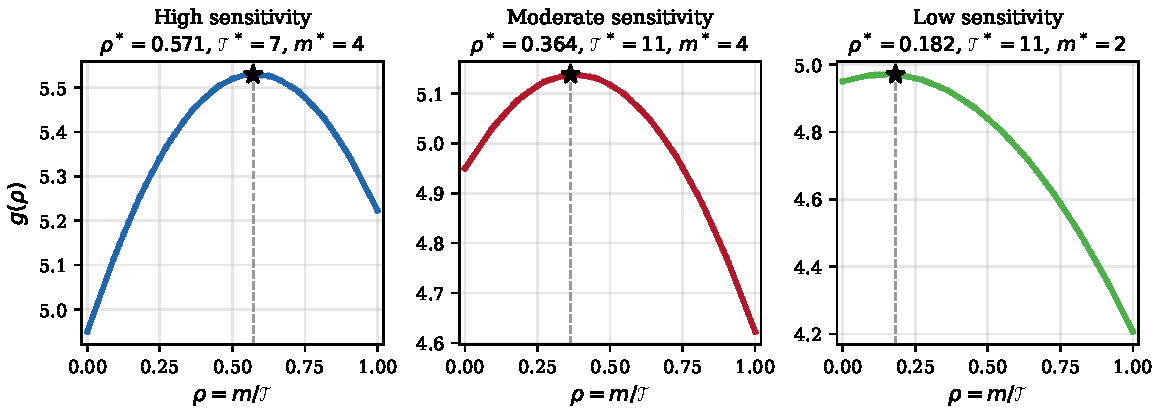
\includegraphics[width=\textwidth]{exp1_g_rho.pdf}
\caption{Promotion frequency in an affine engagement example. The balanced revenue \(g^{\mathrm{aff}}(\rho)\) is continuous and piecewise linear, and the stars mark the maximizing promotion frequency \(\rho^\star\). The parameters are \(\mathcal A=10\), \(p^{L}=1\), \(p^{H}=1.8\), \(\alpha_a^{\mathrm{aff}}=0.25\), and \(\eta_a^{\mathrm{aff}}=\beta_a^{\mathrm{aff}}\). The high, moderate, and low sensitivity profiles are \(\beta_a^{\mathrm{aff}}=0.1(0.85)^a\), \(0.0625(0.88)^a\), and \(0.0375(0.92)^a\), respectively.}
\label{fig:exp1}
\end{figure}
\subsubsection{Heterogeneous lag effects}
\label{sec:affine-location-dependent}
The affine count model assigns the same marginal effect to every remembered promotion. We now allow engagement effects to differ across lags, so promotions one and two periods earlier can have different influences on current demand. This extension distinguishes histories with the same promotion count, so Assumption~\ref{ass:additive-engagement} no longer applies directly. The pairwise revenue representation nevertheless gives a separate condition for balanced optimality.

A related formulation appears in reference price research, where exponential smoothing assigns declining weights to past prices, as in \citet{hardie1993reference}, \citet{kopalle1996reference}, and \citet{popescu2007}. Individual cohort coefficients in our model need not decline with lag. The following result establishes balanced optimality under a discrete convexity condition on the aggregate lag coefficients.

Consider the market share function
\begin{equation}\label{eq:pd-model}
    M_a^{\mathrm{loc}}(d_t,\ldots,d_{t-a})
    =\alpha_a^{\mathrm{loc}}
     +\beta_{a,0}^{\mathrm{loc}}d_t
     +\sum_{j=1}^{a}\beta_{a,j}^{\mathrm{loc}}d_{t-j}.
\end{equation}
The coefficient \(\beta_{a,0}^{\mathrm{loc}}\) measures the current promotion effect, while \(\beta_{a,j}^{\mathrm{loc}}\) measures the effect of a promotion \(j\) periods earlier. Assume all coefficients are nonnegative and
\[
    \alpha_a^{\mathrm{loc}}+\sum_{j=0}^{a}\beta_{a,j}^{\mathrm{loc}}\le1,
\]
so market shares remain in \([0,1]\).

The arrangement condition depends on historical effects aggregated across active cohorts. Define
\[
    \bar\beta_j^{\mathrm{loc}}
    =\sum_{\{a:a\ge j\}}\beta_{a,j}^{\mathrm{loc}},
    \qquad j=1,\ldots,\mathcal A,
\]
and set
\[
    \bar\beta_{\mathcal A+1}^{\mathrm{loc}}
    =\bar\beta_{\mathcal A+2}^{\mathrm{loc}}=0.
\]

\begin{proposition}[Balanced optimality with heterogeneous lag effects]\label{thm:pd-balanced}
If
    \begin{equation}\label{eq:loc-beta-convex}
        \bar\beta_b^{\mathrm{loc}}
        -2\bar\beta_{b+1}^{\mathrm{loc}}
        +\bar\beta_{b+2}^{\mathrm{loc}}\ge0,
        \qquad b=1,\ldots,\mathcal A,
    \end{equation}
    then every balanced cycle maximizes revenue among cycles with the same length and number of promotions.
\end{proposition}

The result follows by expressing the revenue effects of specific lags through promotion combination counts of order two. Write \(Q_b(C)=Q_{b,2}(C)\) and let
\[
    P_j(C)=\sum_{t=1}^{\mathcal T}d_t(C)d_{t-j}(C)
\]
count promotional periods preceded by another promotion \(j\) periods earlier. At fixed \((\mathcal T,m)\), the arrangement component of revenue is
\[
    -\Delta p\sum_{j=1}^{\mathcal A}\bar\beta_j^{\mathrm{loc}}P_j(C).
\]
Using
\[
    P_b(C)=Q_b(C)-2Q_{b-1}(C)+Q_{b-2}(C),
    \qquad Q_0(C)=Q_{-1}(C)=0,
\]
the coefficient on \(Q_b(C)\) becomes
\[
    -\Delta p\left(
        \bar\beta_b^{\mathrm{loc}}
        -2\bar\beta_{b+1}^{\mathrm{loc}}
        +\bar\beta_{b+2}^{\mathrm{loc}}
    \right).
\]
The resulting window contribution is \(F_b(n)=-\Delta p(\bar\beta_b^{\mathrm{loc}}-2\bar\beta_{b+1}^{\mathrm{loc}}+\bar\beta_{b+2}^{\mathrm{loc}})\binom n2\). Its second difference is nonpositive under the stated condition, so the window concavity argument of Theorem~\ref{thm:general-sign-arrangement} gives balanced optimality. Details appear in Section~\ref{app:affine-recency}.

This condition recovers the affine case of Assumption~\ref{ass:additive-engagement} when historical coefficients do not depend on lag. If \(\beta_{a,j}^{\mathrm{loc}}=\beta_a^{\mathrm{aff}}\) for \(j\ge1\), then \(\bar\beta_j^{\mathrm{loc}}=\sum_{a=j}^{\mathcal A}\beta_a^{\mathrm{aff}}\), and
\[
 \bar\beta_b^{\mathrm{loc}}-2\bar\beta_{b+1}^{\mathrm{loc}}
 +\bar\beta_{b+2}^{\mathrm{loc}}
 =\beta_b^{\mathrm{aff}}-\beta_{b+1}^{\mathrm{aff}}.
\]
Thus declining historical slopes are the count model counterpart of the aggregate lag convexity condition.

The finite memory cutoff affects the convexity condition. For a geometric profile \(\bar\beta_b^{\mathrm{loc}}=cr^b\), with \(c>0\), \(0<r<1\), and \(\mathcal A\ge2\), the interior second differences are nonnegative. The condition at \(b=\mathcal A-1\) additionally requires
\[
    \bar\beta_{\mathcal A-1}^{\mathrm{loc}}
    \ge2\bar\beta_{\mathcal A}^{\mathrm{loc}},
\]
which holds when \(r\le1/2\).

\subsection{Reference price channel}
\label{sec:reference-engagement}
The reference price channel has a different historical effect. A past discount lowers the price against which customers evaluate the current offer and can reduce demand at a given current price. We study a linear, loss neutral model and derive its implications for promotion arrangement and frequency.

For \(a\ge1\), let
\[
    r_{a,t}=\sum_{j=1}^{a}w_{a,j}p_{t-j},
    \qquad w_{a,j}\ge0,
    \qquad \sum_{j=1}^{a}w_{a,j}=1,
\]
and consider
\begin{equation}\label{eq:reference-market-share}
    M_{a,t}=u_a-v_ap_t+\gamma_a(r_{a,t}-p_t),
    \qquad v_a,\gamma_a\ge0.
\end{equation}
The market share function is loss neutral because the same coefficient \(\gamma_a\) applies to gains and losses relative to the reference price. At age zero, omit the reference price term and set \(\gamma_0=0\). Parameters are chosen so that market shares lie in \([0,1]\) for every feasible price history. Unequal reference weights distinguish histories with the same promotion count, giving a lag dependent affine model as in Section~\ref{sec:affine-location-dependent}.

With the average reference price, \(w_{a,j}=1/a\), we have \(r_{a,t}=p^H-\Delta p\,y_{a,t}/a\). The market share function then has the additive form \eqref{eq:additive-market-share}, with \(\alpha_a=u_a-v_ap^H\), \(\eta_a=(v_a+\gamma_a)\Delta p\), and
\[
    f_a(y)=\beta_a^{\mathrm{aff}}y,\qquad
    \beta_a^{\mathrm{aff}}=-\frac{\gamma_a\Delta p}{a},
    \qquad a=1,\ldots,\mathcal A.
\]
A strictly negative historical slope violates the engagement assumption. Suppose \(\gamma_a/a\) weakly decreases with age, as it does when reference sensitivity is constant across ages. Then
\[
    \beta_1^{\mathrm{aff}}\le\cdots\le
    \beta_{\mathcal A}^{\mathrm{aff}}\le
    \beta_{\mathcal A+1}^{\mathrm{aff}}=0,
\]
and hence
\[
    \psi_{b,k}
    =-\Delta p\bigl(\beta_b^{\mathrm{aff}}-\beta_{b+1}^{\mathrm{aff}}\bigr)\ge0,
    \qquad 1\le k\le b\le\mathcal A.
\]
Every window contribution \(F_b\) is therefore convex.

\begin{proposition}[Reference price benchmark]\label{prop:reference-constant-price}
Suppose reference prices equal average past prices and \(\gamma_a/a\) weakly decreases with age. A single promotion block maximizes revenue at any fixed cycle length and number of promotions. When frequency is unrestricted, the better constant price is optimal over all feasible infinite price paths.
\end{proposition}

The result follows from Theorem~\ref{thm:general-sign-arrangement} and Proposition~\ref{prop:general-cluster-frequency}. Grouping promotions reduces the adverse effect of earlier discounts on demand during regular price periods. When frequency can also be chosen, a constant price weakly dominates every promotion cycle. The proof appears in Section~\ref{app:reference-engagement} of the supplementary appendix.

This constant price benchmark connects our arrangement analysis to classical reference price findings. \citet{kopalle1996reference} derive conditions for constant or cyclic pricing under asymmetric responses to gains and losses. \citet{popescu2007} establish convergence to a constant price for loss neutral and loss averse demand under their assumptions, with continuously chosen prices and discounted revenue. Proposition~\ref{prop:reference-constant-price} establishes constant price optimality under the stated reference price conditions, two given prices, and long run average revenue.

These arrangement and constant price conclusions also hold for reference prices smoothed exponentially within each cohort from a fixed initial reference, with common reference sensitivity across ages, by the same window convexity argument. The proof appears in \hyperlink{proof-exponential-reference}{Section~\ref*{app:reference-engagement}} of the supplementary appendix.

For general nonnegative reference weights summing to one, the better constant price remains optimal even without the age monotonicity condition. Equation~\eqref{eq:reference-variation-penalty} expresses average cycle revenue as the frequency weighted average of the two constant price revenues minus a nonnegative penalty for price variation. This frequency conclusion does not require convexity of every window contribution and does not by itself establish single block optimality at fixed frequency.
